%TODO:


\documentclass[a4paper]{scrartcl}

\usepackage[utf8]{inputenc}
\usepackage[english]{babel}
\usepackage{lmodern} 
\usepackage[T1]{fontenc}
\usepackage{booktabs}
\usepackage{multirow}
\usepackage{wrapfig}


% PAKETE
\usepackage{siunitx}
\usepackage{graphicx}
\usepackage[usenames,dvipsnames]{xcolor}
\usepackage{placeins}
\usepackage{longtable}
\usepackage{enumitem}
\usepackage{bbm}

\usepackage{amssymb} % math symbols
\usepackage{amsmath} % ams
\usepackage{amsfonts} % mathmatical fonts

% caption indenting
 \usepackage[format=plain,indention=0em,labelfont=bf,margin=1em]{caption} 
 \usepackage{subfig} %subfigures ^^
\usepackage[protrusion=true,expansion=true]{microtype} % denser font, "-" behind line
\usepackage{esint} % nicer double and triple integrals
\usepackage{fancyhdr} % fancy headers
\usepackage[colorlinks=true,linkcolor=black,citecolor=black,filecolor=black,urlcolor=black]{hyperref}



% EINSTELLUNGEN
\sisetup{seperr,repeatunits=false}
\numberwithin{equation}{section}
\numberwithin{figure}{section}
\numberwithin{table}{section}

% EIGENE FUNKTIONEN
\newcommand{\re}{\operatorname{Re}}
\newcommand{\im}{\operatorname{Im}}
\newcommand{\gquote}[1]{\glqq #1 \grqq}

\newcommand{\eq}[2]{\begin{equation}#1\label{#2}\end{equation}}
\newcommand{\eqand}[0]{\hspace{.25cm} \bigwedge \hspace{.25cm}}
\newcommand{\grafik}[2]{\begin{figure}[h]\centering \includegraphics[width=10cm]{#1.eps}  \caption{#2} \label{#1} \end{figure} }
\newcommand{\grafikq}[3]{\begin{figure}[h]\centering \includegraphics[width=10cm]{#1.eps}  \caption[#2]{#3} \label{#1} \end{figure} }
\newcommand{\tbl}[3]{\begin{table}[h]\caption{#1}\label{#2}\begin{center}#3\end{center}\end{table}}
\newcommand{\Abbildung}[1]{\textsl{Abbildung \ref{#1}}}
\newcommand{\AbbildungI}[1]{\textsl{(Abbildung \ref{#1})}}
\newcommand{\Tabelle}[1]{\textsl{Tabelle \ref{#1}}}
\newcommand{\TabelleI}[1]{\textsl{(Tabelle \ref{#1})}}
\newcommand{\Formel}[1]{(\ref{#1})}
\renewcommand{\d}{\mathrm{d}}
\newcommand{\ve}[1]{\mathbf{ #1} }

\title{Ma 5: Dynamical Processes in Lipid Membranes}
\subtitle{Tutor: Dr. P. Chernev}
\author{Benjamin Huber, Carolin Wille}
\date{January 30, 2012}

\begin{document}
\thispagestyle{empty}
\maketitle
\tableofcontents
\clearpage

\section{Introduction}
\subsection{Spectrum}
In order to understand the emission and absorption spectrum of molecules, it is important to know the structure of energy levels and the transitions, which can occur between them. In the Born-Oppenheimer approximation, which is valid if the electronic transitions happen on a much shorter time scale than the changes in the distance of the atomic nuclei, the wavefunction, which describes the state of the molecule factorises in electronic and nuclear components. The components connected to the nuclei include rotation and vibrational states. If the rotational degrees of freedom are suppressed, e.g. if the molecule is embedded in a certain structure, only the vibrational levels are relevant. The transitions, which lead to the emission of visible light are electronic transitions, that are combined with a vibronic transition. In the dipole approximation, that is valid if the wavelength of the emitted light is considerably longer than the atomic radii, the probability amplitude for such a electronic-vibronic transition is given by 
\eq{ P = \langle \Psi'  \mid   \ve {\hat{D}} \mid \Psi \rangle =  \langle \psi_\text{el'} \mid   \ve {\hat{D}_{el}} \mid \psi_\text{el} \rangle \langle \psi_\text{s'} \mid \psi_\text{s} \rangle \langle \psi_\nu'  \mid  \psi_\nu \rangle \; .} {transition }
The spatial overlap of the two vibronic state nuclear wavefunction squared  $\lvert \langle \psi_\nu'  \mid  \psi_\nu \rangle \rvert ^2$ is called the Franck-Condon factor and expresses the fact, that transitions are more likely to occur, if the position of the nuclei remain more or less the same during an electronic transition. This is called the Franck-Condon principle and is illustrated in figure \ref{condon}.

An excited state can relax into its groundstate via different intermediate processes. Radiation less transitions, which can occur via exchange of phonons or collisions with other atoms and molecules are usually very fast, because the energy difference between those states is typically small. Thus, an excited vibronic state decays fast into its ground state. The relaxation of the electronic excited state and vibronic ground state into the electronic ground state and excited vibronic state (cf. fig \ref{jablonsk}) is called fluorescence. As its emitted photons are typically in the visible light regime, fluorescence is a luminescent process. The other luminescence, which can occur is phosphorescence, where the system decays first into a state, which is forbidden according to spin selection rules. Such a transition, where the electron spin changes is called intersystem crossing. The decay into ground state is again forbidden according to the dipole selection rules. Therefore, the lifetime if this state is very high, which leads to the phenomenon of light emission long after absorption.

Considering two electronic states with similar vibronic structure, the absorption spectrum is symmetric to the fluorescence spectrum as a consequence of the Franck-Condon principle (cf. \ref{condon}). This symmetry can be detected in the experiment although the equal spacing of the energy levels is an idealization, meaning that the real structures do not look exactly symmetric.


\begin{figure}
\centering
\subfloat[][Franck-Condon Principle]{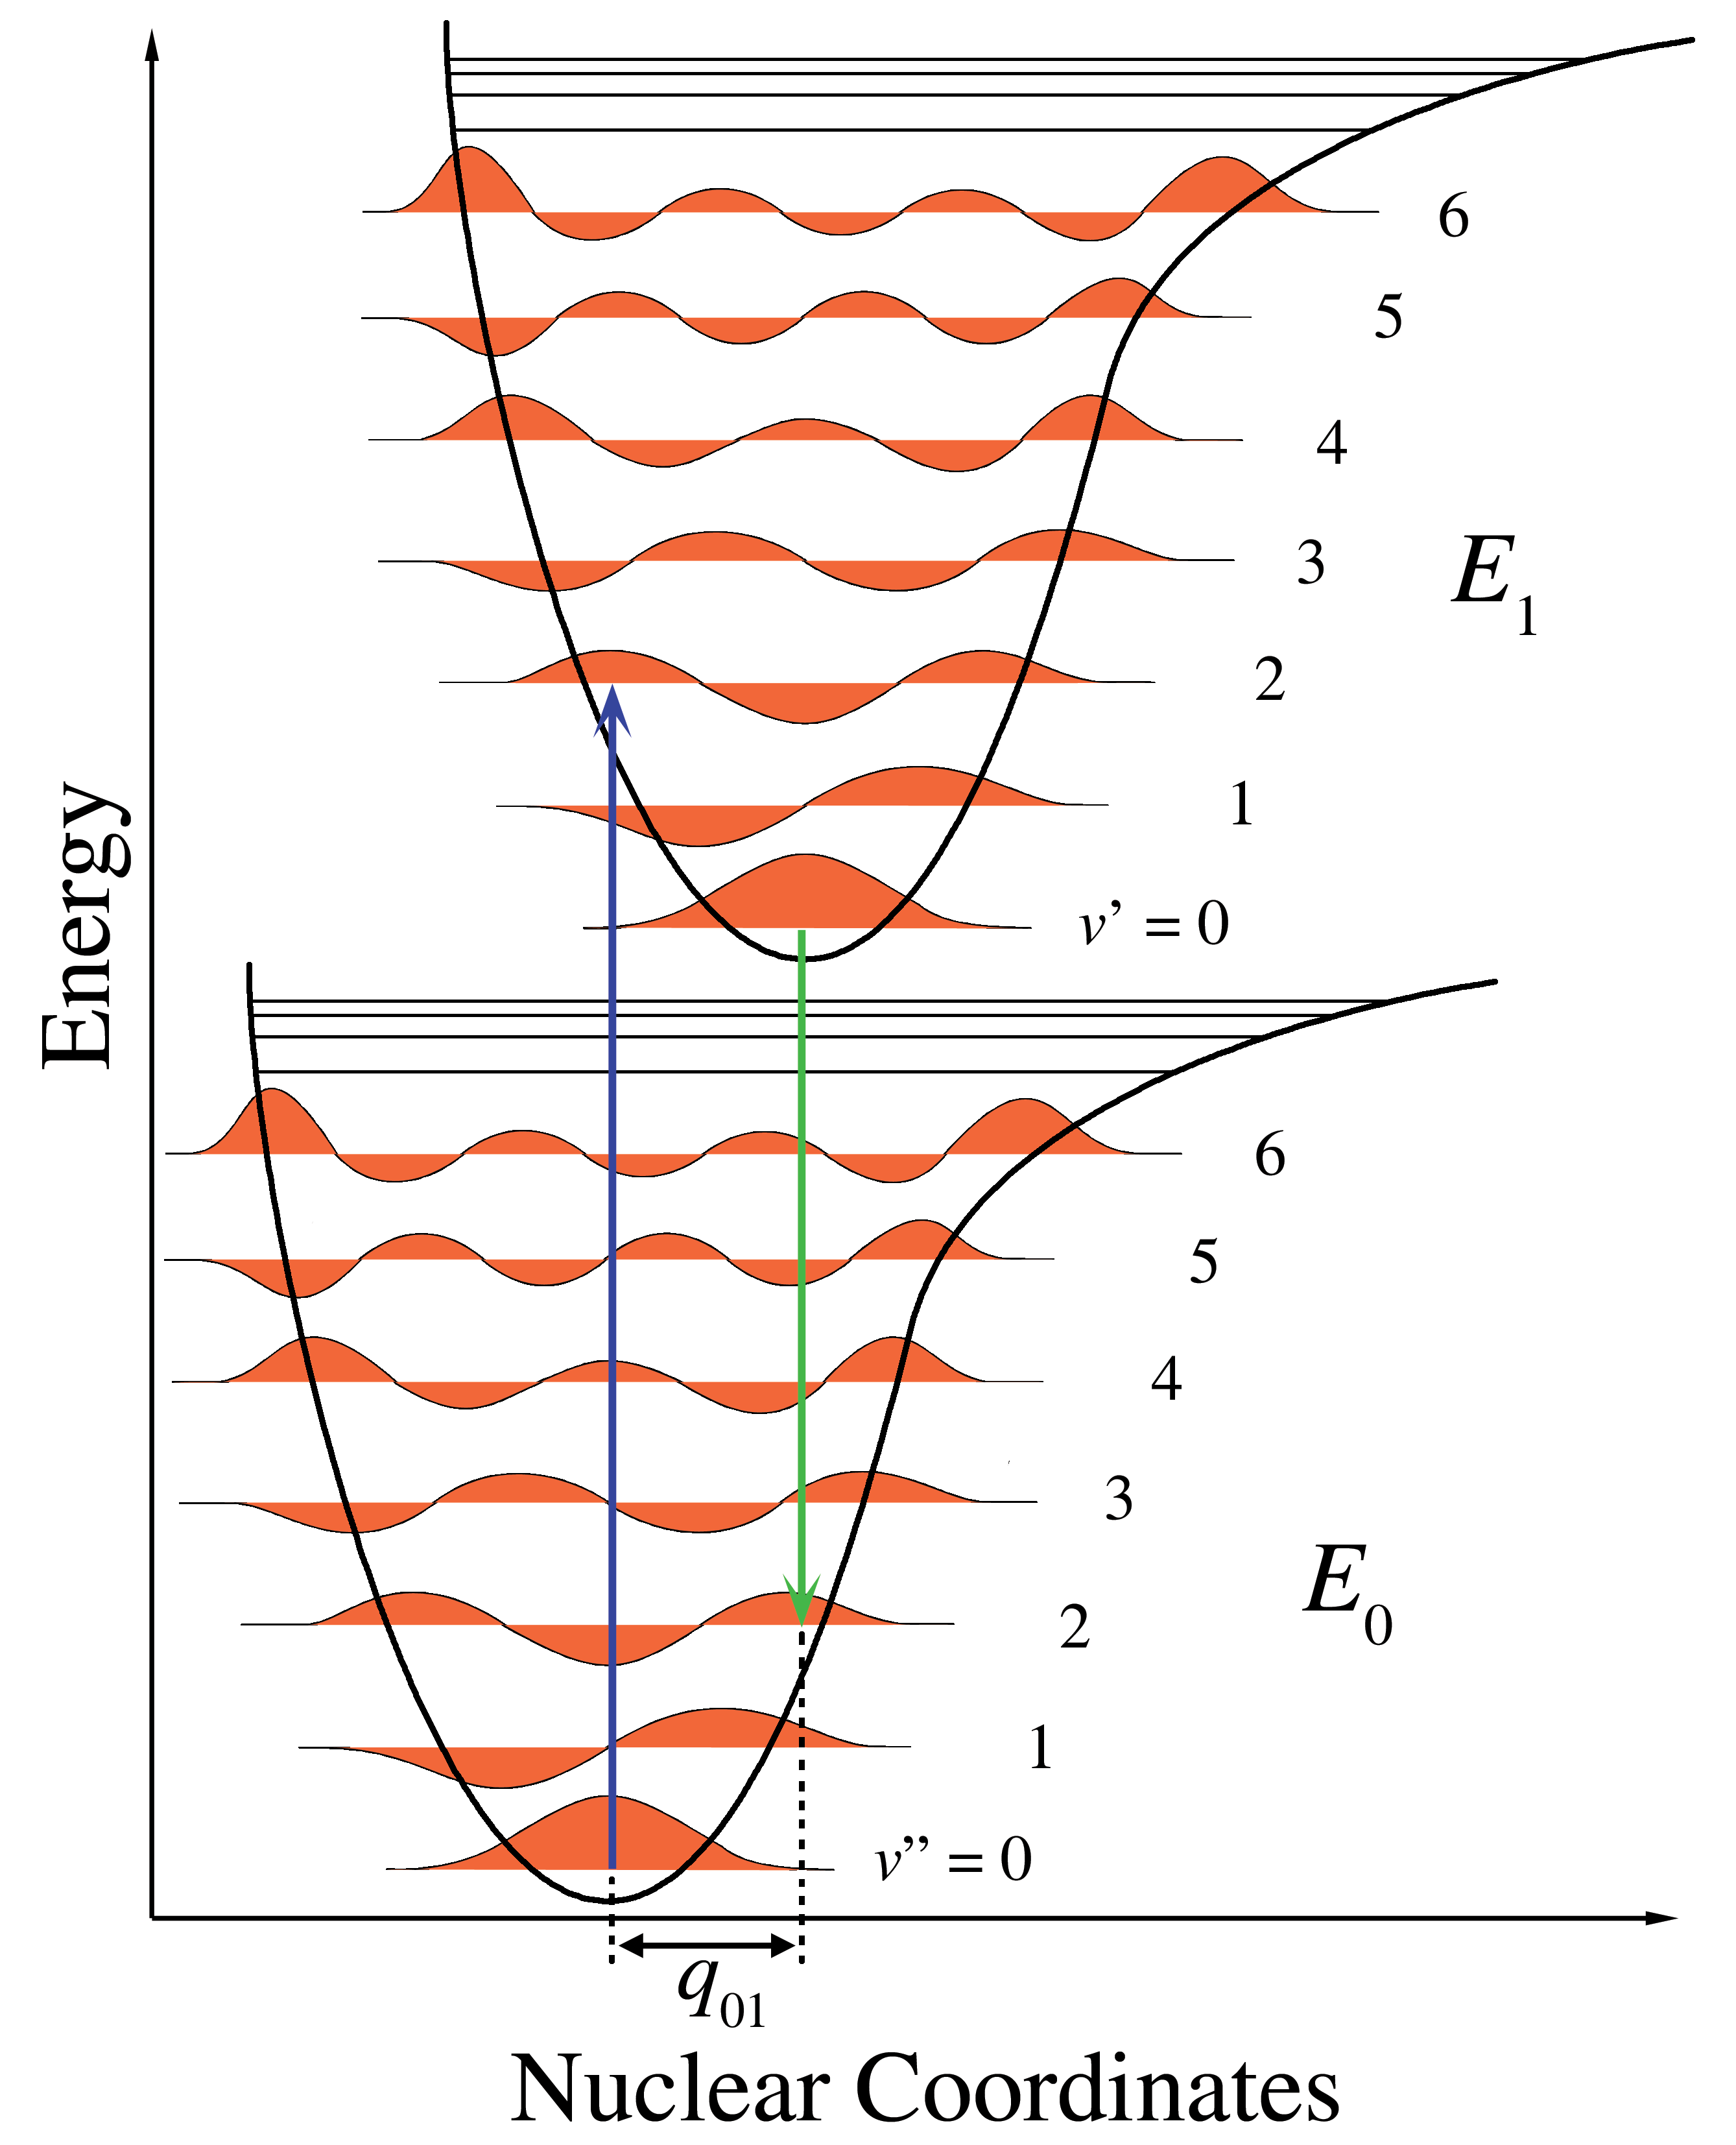
\includegraphics[width=0.5\linewidth]{img/condon.png}}
\hfill
\subfloat[][Spectrum]{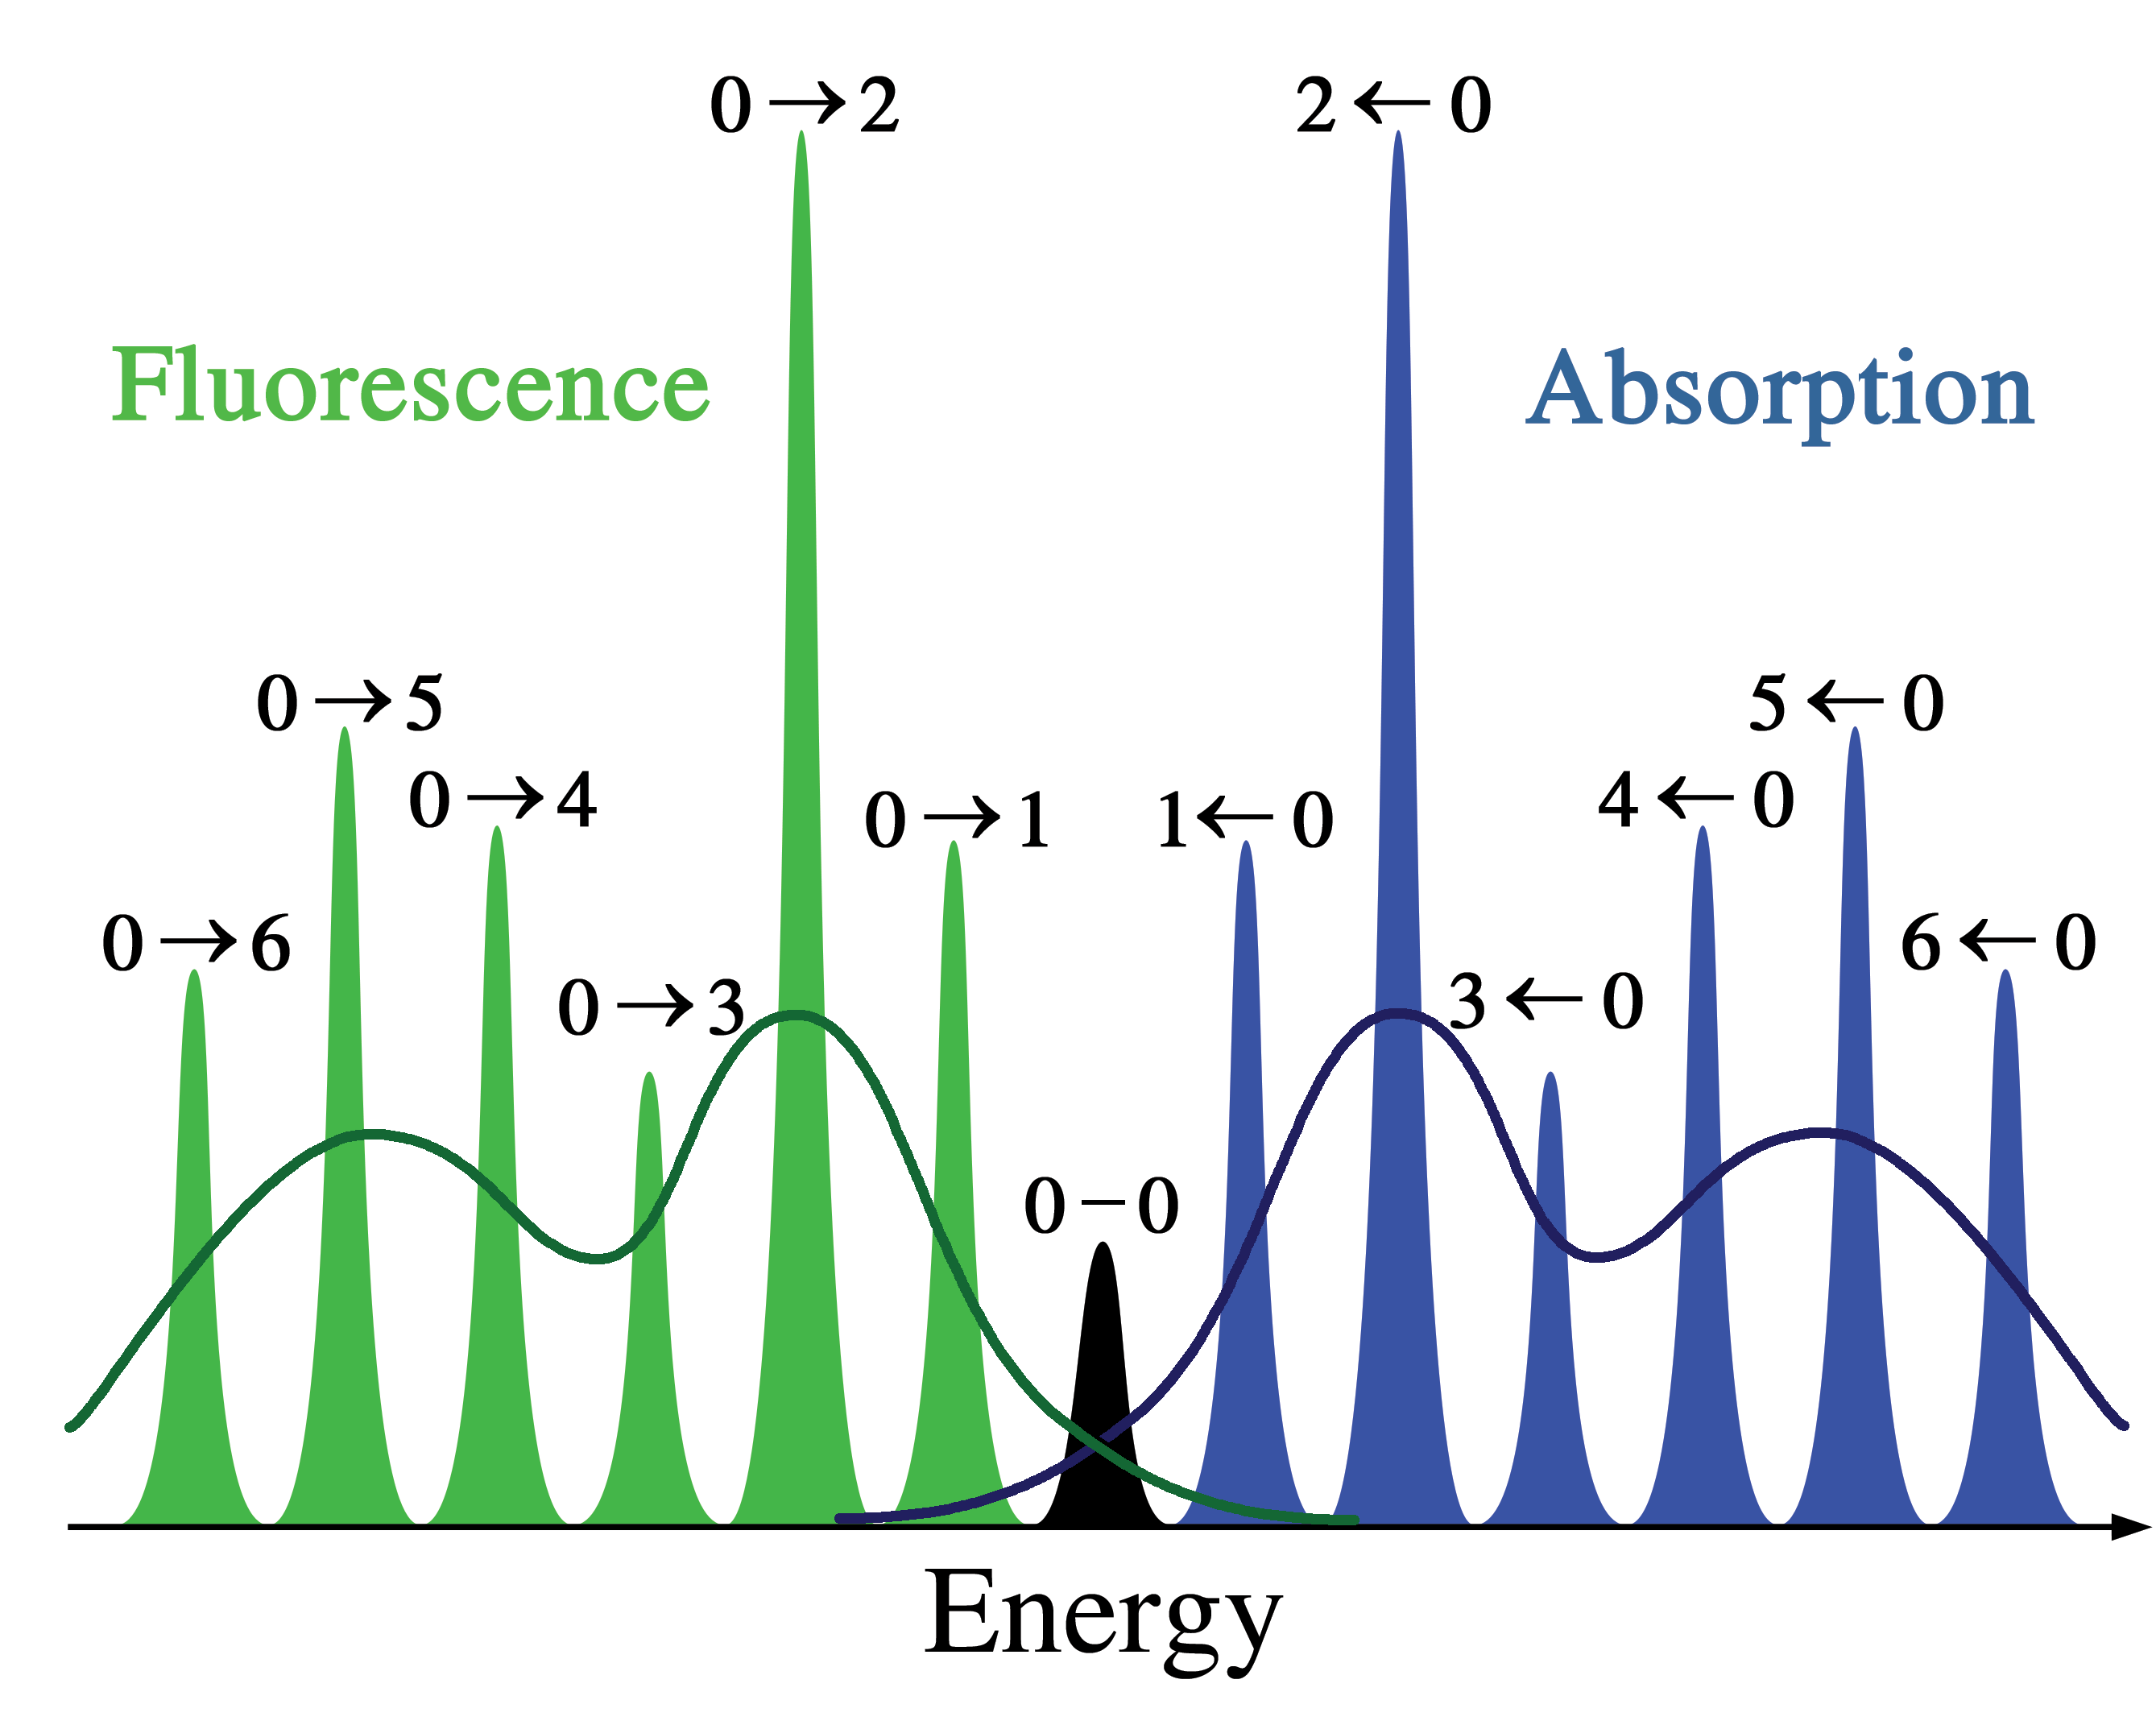
\includegraphics[width=0.5\linewidth]{img/absorptionemission.png}}

\subfloat[][]{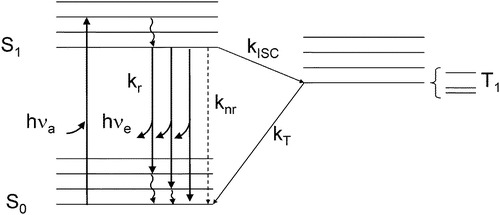
\includegraphics[width=0.7\textwidth]{img/Jablonski.jpg}}
\caption{ \small \textbf{(a)} Illustration of the Franck-Condon principle, which is a direct consequence of the Born-Oppenheimer approximation and states, that those electronic-vibraonic transitions are favored, which leave the inter-nuclei distance mostly unchanged. \textbf{(b)} Symmetric structure of an absorption and fluorescence spectrum. Sharp peaks will be visible in dilute gases, while in liquids and solids the peaks are widened. \footnotesize Source: \url{http://en.wikipedia.org/wiki/Franck-Condon_principle}}
\label{condon}
\end{figure}


\begin{figure}
\centering
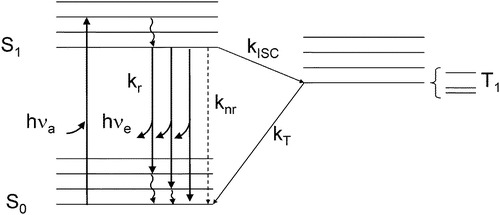
\includegraphics[width=0.5\textwidth]{img/Jablonski.jpg}
\caption{\small Jablonski diagramme of possible transitions. \footnotesize Source: \url{http://web.uvic.ca/ail/techniques/epi-fluorescence.html} }
\label{jablonsk}
\end{figure}

\clearpage
 \bibliographystyle{unsrt}
\bibliography{bib}



\end{document}


